\section{Methodology}

\subsection{Data Preparation}

PHQ8 values are organized to multiclass \cite{kroenke2001phq} based on the depression severity, and these severitities into binary values (non depression, depression) \cite{kroenke2009phq}. Table \ref{tab:phq8_severity} shows how these values are organized. In case of EATD the the SDS index is categorized by and it is mapped to binary categories as it shown in Table \ref{tab:sds_index_classification}.

\begin{table}[H]
    \centering
    \caption{Severity levels according to the PHQ-8 score.}
    \begin{tabular}{|c|c|c|}
    \hline
    \textbf{PHQ-8 Scores} & \textbf{Severity} & \textbf{Binary} \\
    \hline
    0--4 & Non depression & 0 \\
    5--9 & Mild & 0 \\
    10--14 & Moderate & 1 \\
    15--20 & Moderately severe & 1 \\
    21-- & Severe & 1 \\
    \hline
    \end{tabular}
    
    \label{tab:phq8_severity}
\end{table}

\begin{table}[H]
    \centering
    \caption{Depression severity levels based on SDS index scores with corresponding binary classification.}
    \begin{tabular}{|c|c|c|}
    \hline
    \textbf{SDS Index} & \textbf{Severity} & \textbf{Binary} \\
    \hline
    0--49 & Normal & 0 \\
    50--59 & Mild & 1 \\
    60--69 & Moderate & 1 \\
    70--100 & Severe & 1 \\
    \hline
    \end{tabular}
    
    \label{tab:sds_index_classification}
\end{table}

\subsection{Audio Features}
Speech contains various acoustic characteristics that can be analyzed for depression detection. While numerous features exist for audio analysis, this study primarily focuses on two key representations: Mel-Frequency Cepstral Coefficients (MFCC) and Mel Cepstral Coefficients (MCC). Both representations use 40 frequency bands, where each band captures a specific range of frequencies, creating a detailed "fingerprint" of the audio signal. These 40 bands are distributed logarithmically across the frequency spectrum, meaning lower frequencies (which are crucial for human speech) are represented with finer detail than higher frequencies.

Figure \ref{fig:mfcc_mcc} shows the MFCC and MCC representation of the word "Depression" \footnote{Audio record, recorded by me}. In these visualizations, each of the 40 bands appears as a row, with colors indicating the intensity of the signal at different time points. The MFCC representation captures the spectral features of the audio signal, while the MCC representation emphasizes the cepstral features, providing a more detailed view of the audio signal's temporal dynamics. The choice of feature representation is crucial for model performance, as it determines the information available to the model for classification.

\begin{figure}[H]
    \centering
    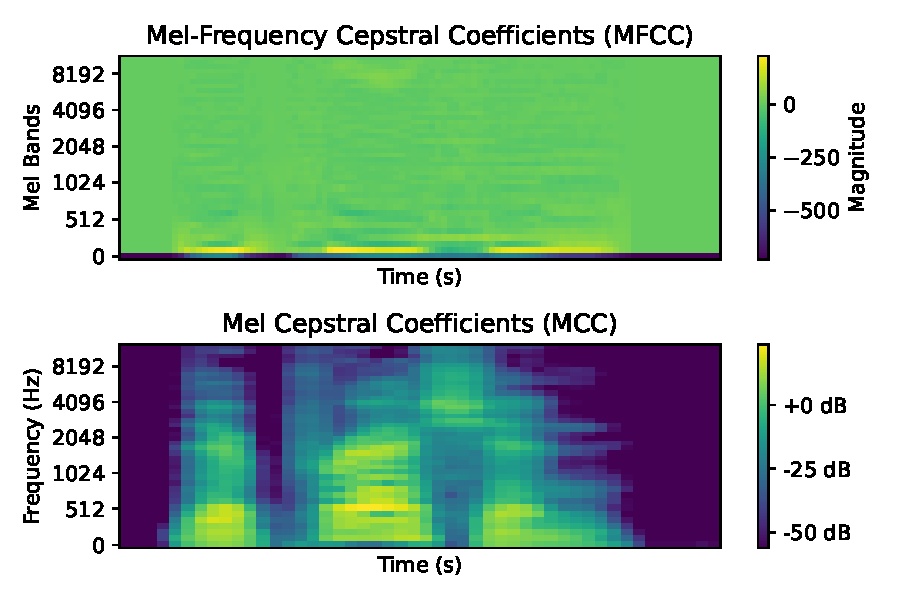
\includegraphics[width=0.45\textwidth]{vis_pdf/mfcc_mcc_comparison.pdf} % Adjust the scale to fit the page
    \caption{Visual comparison of MFCC and MCC representations for the word "Depression", highlighting their distinct audio feature emphases. Length of the audio signal is 1 seconds, sampling rate is 24Khz, it generates a 100 long MFCC and MCC.}
    \label{fig:mfcc_mcc}
\end{figure}

\subsubsection{MFCC}

MFCCs are pivotal for analyzing the power spectrum of audio signals, particularly in tasks like speech recognition. MFCCs provide a representation of sound that approximates human auditory perception, with the mel scale mapping onto the frequency sensitivity patterns of the human cochlea \footnote{\url{https://cdn.britannica.com/04/14304-050-1A5E3289/structures-outer-ear.jpg}} . The extraction process has several steps: First, the audio signal is transformed from a time-based wave into its frequency components using the Fast Fourier Transform. These frequencies are then mapped onto the mel scale - a special scale that gives more attention to lower frequencies (like human speech) and less to higher frequencies (like high-pitched whistles), just as our ears do naturally. This mapping happens through a mel filter bank, which works like a series of overlapping filters that focus on different frequency ranges, similar to how different parts of our inner ear respond to different pitches. The outputs are then adjusted (logged) to match how we perceive loudness, since humans don't perceive sound intensity linearly - a whisper to normal speech feels like a smaller jump than normal speech to a shout. Finally, these features are mathematically processed (using a Discrete Cosine Transform \cite{wikidct}) to create the final MFCCs that effectively capture the key characteristics of the sound (the result is visualised on the first image \ref{fig:mfcc_mcc}).

\subsubsection{MCC}
Similar to MFCCs, MCCs also represent audio characteristics, but with a key difference in how they process the signal. While MFCCs use filter banks to mimic human hearing, MCCs employ a more direct mathematical approach that can capture subtle variations in speech: if MFCCs are like hearing sound through human ears, MCCs are like looking at sound through a precise scientific instrument. This makes MCCs particularly effective at capturing the unique characteristics of human voice, especially in tasks where subtle voice variations matter.

\subsection{Feature Extraction Process}
For the DAIC dataset, audio segments containing patient speech were isolated and processed. Each segment underwent feature extraction to compute either MFCC or MCC representations. For the Decision Tree model, statistical measures (minimum, average, and maximum values) were calculated across all segments for each patient. For the CNN model, the raw MFCC and MCC spectra were processed in 200-frame chunks.

For the EATD dataset, each participant recorded three different sentences: one with neutral emotion, one with positive emotion, and one with negative emotion. Each of these single-sentence recordings underwent the same feature extraction process as the DAIC dataset, with statistical measures computed for each sentence separately.

---------------


% This approach ensures that while no preprocessing is applied to clean the audio, the data retains its natural characteristics, potentially influencing the robustness and generalizability of the depression detection models.


% MODELS

\subsection{Models}
Two model will be built for the evaluation. One is a decission tree (DT) another one is a Transformer-CNN-CNN (TCC)\cite{yin2023depression}.

\subsubsection{Decision Tree}

The methodology employed for optimizing the DT classifier involves an integrated approach to feature selection and tree depth configuration. The objective is to enhance model performance while preventing overfitting. Feature selection was performed using three techniques to evaluate their effectiveness in identifying the most predictive features:

\begin{enumerate}
    \item \textbf{ANOVA F-value:} Analyzes the variance among classes to identify features that significantly differentiate between them. This method calculates the F-value for each feature to determine its impact on classification accuracy, prioritizing those with higher values for model inclusion.
    \item \textbf{Mutual Information (MI):} Measures the dependency between the features and the target variable, crucial for capturing nonlinear relationships.
    \item \textbf{Random Forest Feature Importance (RF):} Utilizes the Random Forest algorithm to estimate the usefulness of each feature based on the impurity reduction it brings to the model.
\end{enumerate}

These methods were chosen to provide a comprehensive analysis of feature relevance from both statistical and machine learning perspectives. The Decision Tree's depth was then tuned to find the optimal balance that yielded the highest accuracy on the validation set, using the most predictive features identified by the feature selection process.

To mitigate the risk of overfitting, I methodically investigated a range of tree depths from 1 to 19, while also varying the number of top-ranked features from 1 to 29. This approach allowed me to assess the model’s performance at each depth, using different subsets of top features to determine the optimal combination that enhances model accuracy without overfitting. The evaluation metrics include F1-score \cite{gfg_f1score} and accuracy, with a particular emphasis on the weighted average F1-score due to the imbalanced nature of our dataset. This metric adjusts for label imbalance by weighting the F1-score of each class by its support (the number of true instances for each label). This approach ensures that my model's performance is robust across different class distributions and provides a more reliable indication of its generalization ability.

The final model parameters—optimal feature count and tree depth—are selected based on their performance on the development set, aiming to maximize the weighted average F1-score while maintaining generalizability across the dataset.

\subsubsection{Convolutional Neural Network}

I adapted three CNN models based on the studies highlighted in the literature review. Among these, the TCC model underwent a more detailed analysis. It integrates two parallel CNN streams with a transformer stream. This design effectively combines local and global information processing capabilities. Specifically, the parallel CNN streams are utilized to extract local features from the input, while the transformer stream, employing linear attention mechanisms, captures the temporal dynamics. This configuration is particularly optimized for handling the complexities of the dataset.

Each CNN stream processes the input independently to capture diverse aspects of the data, and the transformer stream analyzes the sequence as a whole. The outputs of these streams are then fused, combining their feature spaces to enhance the model's prediction accuracy. This fusion happens in a fully connected layer that integrates learned features before the final classification layer.

Modifications include adjusting the dimensionality of the input features and streamlining the transformer's attention mechanism to reduce computational complexity.

